\documentclass[a4paper,11pt,titlepage]{report}
\usepackage[english]{babel}
\usepackage[margin=3cm]{geometry}
\usepackage[T1]{fontenc}
\usepackage[utf8]{inputenc}
\usepackage{lmodern}
\usepackage[sorting=none]{biblatex}
\usepackage{graphicx}
\usepackage{fancyhdr}
\usepackage[textfont={small,it},labelfont=bf,labelsep=endash]{caption}
\usepackage[table]{xcolor}
\usepackage{verbatim}
\usepackage[toc,page]{appendix}
\usepackage{url}
\usepackage{amsmath}
\usepackage{multicol}	% allow multi column environemnt
\usepackage{float} % forced position of figures/tables etc.
\usepackage{acronym}
\usepackage{rotating}
\usepackage{titling}
\usepackage{bibcheck}
\usepackage[center]{subfigure} % make it possible to include more than one captioned figure/table in a single float
\usepackage[pdfstartview=FitH,pdfborder={0 0 0},bookmarks]{hyperref}
\usepackage{memhfixc}
\usepackage{placeins}
\usepackage{longtable} % multi-page table environment
\usepackage{tabularx}
%\usepackage[pdftex]{hyperref}
\hypersetup{colorlinks=true, linkcolor=black, citecolor=black, filecolor=black, urlcolor=black,
pdftitle={U-SPACE Critical Design Report}}


\graphicspath{{./figures/}}	% look for graphic files in the "figures" subfolder

\definecolor{tableshade}{HTML}{E8E8E8}
\linespread{1.3}

% define the page headers and footers
\fancyhead{}
\fancyhead[RE,RO]{\parbox[b]{10cm}{\raggedleft U-SPACE\\ \today}}
\fancyhead[LE,LO]{\parbox[b]{10cm}{\docreference \\ \title }}
\renewcommand{\headrulewidth}{0.4pt}
\fancyhfoffset{1cm}
\addtolength{\headheight}{1cm}
\fancyfoot{}
\fancyfoot[C]{\thepage}
\renewcommand{\footrulewidth}{0.4pt}
\newcommand{\rr}{\raggedright} % to use for force left-align in multi-row table cells
\newcommand{\tn}{\tabularnewline} % to use for making the above work :-)

\bibliography{references} % include .bib file for citations

% PLEASE FILL IN THE RELEVANT INFORMATION BELOW:
%
\def\authors{ \vspace{-1.0em}
\begin{tabbing}
Omair \textsc{Sarwar} \hspace{2.5em} \= Pedro \textsc{Cervantes} \\
Morten \textsc{Olsen} \> Jan \textsc{Sommer}
\end{tabbing}
}
\def\docversion{DRAFT}					% Possible versions are: DRAFT, REVIEW or RELEASED
\def\docreference{USPACE-FR-00}	% -00 = DRAFT,  -A1 = 1st release,  -A2 = 1st release with minor updates, -B1, = 2nd release
\def\title{Final Report}


\begin{document}

\input{titlepage}

\pagestyle{plain}
\pagenumbering{roman}

\thispagestyle{plain}
\chapter*{Normative References}
\markboth{Normative References}{Normative References}
\addcontentsline{toc}{chapter}{\protect\numberline{}Normative References}
%
\begin{table}[H]
\centering
\caption{Normative References for this document}
\label{tab:normative_references}
\begin{tabular}{lll}
\hline
\textbf{Document title} & \textbf{Doc. Ref. No.} & \textbf{Doc. status}\\
\hline
Critical Design Report & USPACE-CDR-A2 & Released\\
\hline
\end{tabular}
\end{table}
%
\newpage
%
\thispagestyle{plain}
\chapter*{Document Change Record}
\markboth{Document Change Record}{Document Change Record}
\addcontentsline{toc}{chapter}{\protect\numberline{}Document Change Record}
%
%
\begin{table}[H]
\centering
\caption{Document Change Record for this document}
\label{tab:document_change_record}
\begin{tabular}{p{0.22\textwidth}p{0.18\textwidth}p{0.49\textwidth}}
\hline
\textbf{Doc. version} & \textbf{Change date} & \textbf{Change Description}\\
\hline
USPACE-CDR-A1 & 11 Sep. 2012 & 1st release\\
\hline
\end{tabular}
\end{table}
\thispagestyle{plain}
\chapter*{Acronyms}
\markboth{Acronyms}{Acronyms}
\addcontentsline{toc}{chapter}{\protect\numberline{}Acronyms}

\begin{multicols}{2}
\begin{acronym}
\acro{ADS}{Attitude Determination System}
\acro{BCR}{Battery Charge Regulator}
\acro{BJT}{Bipolar Junction Transistor}
\acro{CC}{Constant Current}
\acro{CDR}{Critical Design Review}
\acro{CM}{Current Mode}
\acro{COTS}{Commercial Of-The-Shelf}
\acro{CPU}{Central Processing Unit}
\acro{DCM}{Discontinuous Conduction Mode}
\acro{DM}{Development Model}
\acro{DSP}{Digital Signal Processor}
\acro{ECSS}{European Cooperation for Space Standardization}
\acro{EGSE}{Electrical Ground Support Equipment}
\acro{EKF}{Extended Kalman Filter}
\acro{EMC}{Electromagnetic Compatibility}
\acro{EMI}{Electromagnetic Interference}
\acro{EPS}{Electrical Power System}
\acro{ESC}{Electronic Speed Control}
\acro{ESR}{Equivalent Series Resistor}
\acro{FM}{Flight Model}
\acro{FRR}{Flight Readiness Review}
\acro{GPS}{Global Positioning System}
\acro{$I^2C$}{Inter-Integrated Circuit}
\acro{IC}{Integrated Circuit}
\acro{IRF}{Swedish Institute of Space Physics}
\acro{ITPU}{Imaging and Tracking Payload Unit}
\acro{ITU}{International Telecommunication Union}
\acro{LDO}{Low-dropout}
\acro{LiPo}{Lithium-Polymer}
\acro{LTU}{Lule\r{a} University of Technology}
\acro{MCC}{Motor Control and Communication}
\acro{MCU}{Micro-Controller Unit}
\acro{MEA}{Main Error Amplifier}
\acro{MGSE}{Mechanical Ground Support Equipment}
\acro{MOSFET}{Metal-Oxide-Semiconductor Field-Effect Transistor}
\acro{MPP}{Maximum Power Point}
\acro{MPPT}{Maximum Power Point Tracking}
\acro{MPPTU}{Maximum Power Point Tracking Unit}
\acro{MSE}{Mechanical Structure and Envelope}
\acro{NTC}{Negative Temperature Coefficient}
\acro{OpAmp}{Operational Amplifier}
\acro{PCB}{Printed Circuit Board}
\acro{PDR}{Preliminary Design Review}
%\acro{SA}{Solar Array}
\acro{PSA}{Pressure Sensitive Adhesive}
\acro{PTC}{Positive Temperature Coefficient}
\acro{PWM}{Pulse Width Modulation}
\acro{RHPZ}{Right Half Plane Zero}
\acro{SAR}{Solar Array Regulator}
\acro{SD}{Secure Digital}
\acro{SMD}{Surface-Mount Device}
\acro{SoC}{System on Chip}
\acro{SPA}{Solar Powered Airship}
\acro{SSC}{Swedish Space Corporation}
\acro{TBD}{To Be Decided}
\acro{U-SPACE}{Unmanned Solar Powered Airship Concept Evaluation}
\acro{UART}{Universal Asynchronous Receiver/Transmitter}
\acro{UAS}{Unmanned Aircraft System}
\acro{UAV}{Unmanned Aerial Vehicle}
\acro{USB}{Universal Serial Bus}
\acro{UVLO}{Under-Voltage Lock-Out}
\end{acronym}
\end{multicols}


\markboth{List of Figures}{List of Figures}
\addcontentsline{toc}{chapter}{\protect\numberline{}List of Figures}
\listoffigures
\newpage

\markboth{List of Tables}{List of Tables}
\addcontentsline{toc}{chapter}{\protect\numberline{}List of Tables}
\listoftables
\newpage

\tableofcontents
\newpage
\acresetall	%reset acronyms which is otherwise used in list of figures or tables
\clearpage %reset page numbers
\pagenumbering{arabic}
\pagestyle{fancy}

\newpage
\chapter{Introduction}
\label{chap:introduction}

Short description of the entire project, including motivation

\section{Hardware}
\label{sec:intro_hardware}

Description of the hardware, including a block diagram

\section{Software}
\label{sec:intro_software}

Description of software, including operational modes
\newpage
\chapter{Design Changes}
\label{chap:design_changes}
% what major design changes have been introduced since the CDR report? Argument why these changes were necessary. Also, will be good to include test results (functionality, weight, performance etc.) which are not documented in the CDR report.
%
%
\section{Project Schedule, Resources and Goals}
\label{sec:project_changes}
%responsible: Morten
%
As previously stated in [CDR ref], the U-SPACE project was initially substantially delayed due to bureaucratic challenges in course registrations and subsequent release of project budget. This resulted in a reformulation of the system concept going from a custom designed helium envelope to a \ac{COTS} blimp provided by Esrange Space Center.

In June 2012, many of the U-SPACE team members left Kiruna to pursue summer internships and prepare for their 3rd semester outside Sweden. Work on the project over the summer holiday was restricted since Lars Jakobsson (LTU technician) was unavailable thus making ordering of new components impossible. Work on U-SPACE began again in September 2012, when Jan and Pedro returned to Sweden and Omair officially joined the project. At this point, Morten took over the full project management responsibilities and also remained responsible for the power subsystem, Jan became the lead responsible for the attitude sensors and payload, Omair responsible for all on-board telemetry handling, telecommunication and ground station and Pedro responsible for the mechanical structure and motors.

Since the sun sits very low on the horizon during autumn in Kiruna and is almost completely absent during winter, it was decided, for the first prototype, not to implement the solar array and related electronics. Instead the goal would be to realize an indoor battery powered flight. This also reduced the work load as was required due to the fewer people now working on the project.

Weekly status meetings were held with project supervisors, but internal meetings were only held on a need-basis since the group just counted four people and were often already sitting together in the Viking project room. 
Due to some misunderstandings of the initial budget, it was approved by the supervisors to increase the project budget for the four remaining students from 2000 SEK to 2500 SEK per student. 


\section{Electrical Power Subsystem}
%responsible: Morten
%
Due to the issues discussed in section \ref{sec:project_changes}, the solar cells were not ordered. However, it is still believed that the cells discussed in [ref to CDR] are suitable for this project.
%
%
In the final circuity layouts, it was decided to place the \ac{BCR} and \ac{SAR} on separate \acp{PCB}. Additionally, a small temperature sensor board was built. The following sections describe the features and circuit diagrams of each of these boards.
%
%
\subsection{Battery}
%
%Challenges in thermal design to achieve specifications on battery. A passive design has been made. Specify test results. Suggestion to add a heater or have a winter + summer configuration of the insulation.
%
During testing of a thermal design, one Li-ion battery underwent a heavy discharge and subsequently showed clear indication of damage (swallowing of the battery pack). There was no immediate danger, however the incidence learned us that it is important that everyone working with Li-ion batteries knows about its safe use and limitations. Li-ion fires are almost impossible to put out. Only useful method is to cover the battery in sand why we recommend LTU to put available a bucket of sand and/or establish a fire proof area/table for working with Li-ion batteries.
%
%
\subsection{Battery Charge Regulator}
%
Table \ref{tab:BCR_features} lists the features of the final \ac{BCR}.
%
\begin{table}[H]
\centering
\caption{Features of developed \ac{BCR}}
\label{tab:BCR_features}
\begin{tabular}{p{0.35\textwidth}p{0.2\textwidth}p{0.4\textwidth}}
\hline
\textbf{Feature/Specification} & \textbf{Value} & \textbf{Comments}\\
\hline
Max output current & 20 A & All outputs combined \\
Output voltage & 6-8 V & Unregulated \\
Input voltage & 9.2-9.5 V & Higher voltage may lead to overheating\\
Weight & ??? & \\
Under voltage protection & $V_{BATT}$ < 6.0 V & Only cuts off motor power outputs \\
Short-circuit protection & $I_{SC}$ > 15 A & Only on motor power outputs \\
Thermal monitoring and charge cut-off & & \\
Automatic charge control & - & Constant current or voltage and trickle charge\\
Charge inhibit by telecommand & & \\
Power cut-off by telecommand & & Only motor power outputs\\
Charge status telemetry & &\\
Charge/discharge current monitoring & & \\
Battery cells voltage monitoring & & \\
\hline
\end{tabular}
\end{table} 
%
The main changes to the \ac{BCR} include added telemetries, telecommands and protection circuits.
%
%
\subsubsection*{Increasing BCR Power Output}
The chosen Li-ion battery can supply up to 66 A continuously or 88 A burst. The main limitation of the \ac{BCR} power output is due to current ratings on the power diode (20 A), power connectors (19 A) and wires (19 A or 11.5 A when using ECSS derating[ref to ECSS]). PCB trace thickness may also become impractically thick at higher currents. 
To increase the output power rating, the best and first option is to use a higher battery voltage by connecting several batteries in series (or using a higher voltage battery pack with more cells in series). 
The current rating can also be increased by using higher power connectors, thicker wire or several wires in parallel, higher power diodes or two diodes in parallel and using thicker PCB copper tracing, reducing trace length, increasing trace width and improving the thermal layout (adding lots of heat sinks and thermal connections).
%
%
All \ac{BCR} functionalities have been tested and verified at room temperature conditions.
%
\begin{figure}[H]
\begin{minipage}[t]{\linewidth}
\centering
\includegraphics[width=0.7\textwidth]{figures/fig_BCR_top}
\end{minipage}
\vspace{2mm}
\begin{minipage}[t]{\linewidth}
\centering
\includegraphics[width=0.7\textwidth]{figures/fig_BCR_bottom}
\end{minipage}
\caption{Battery Charge Regulator}
\label{fig:BCR_top_bottom}
\end{figure}
%
\begin{figure}[H]
\centering
\includegraphics[width=\textwidth]{figures/fig_Schematic_BCR}
\caption{Schematic of the \acl{BCR}}
\label{fig:BCR_Schematic}
\end{figure}
%
%
\subsection{Solar Array Regulator}

5.0V(regulated), 3.3V(regulated),

Inclusion of 3.3V regulated output - mainly due to limitations on BeagleBoard which is not compatible with 5V?

SAR not implemented due to time limitation.

MPPT not implemented due to time limitation.

Components for DC-DC converter already ordered.

Additional telemetry data outputs added for SAR.

\begin{figure}[H]
\begin{minipage}[t]{\linewidth}
\centering
\includegraphics[width=0.7\textwidth]{figures/fig_SAR_top}
\end{minipage}
\vspace{2mm}
\begin{minipage}[t]{\linewidth}
\centering
\includegraphics[width=0.7\textwidth]{figures/fig_SAR_bottom}
\end{minipage}
\caption{Battery Charge Regulator}
\label{fig:SAR_top_bottom}
\end{figure}

\begin{figure}[H]
\centering
\includegraphics[width=\textwidth]{figures/fig_Schematic_SAR}
\caption{Schematic of the \acl{SAR}}
\label{fig:SAR_Schematic}
\end{figure}


\subsection{Temperature Sensor Board}


\begin{figure}[H]
\centering
\includegraphics[width=0.7\textwidth]{figures/fig_Temp_top}
\caption{Temperature Sensor Board}
\label{fig:TS_top}
\end{figure}

\begin{figure}[H]
\centering
\includegraphics[width=\textwidth]{figures/fig_Schematic_TS}
\caption{Schematic of the Temperature Sensor Board}
\label{fig:Schematic_TS}
\end{figure}


\section{Mechanical Structure and Envelope}
%responsible: Pedro 

\section{Motor Control and Communication}
%responsible: Pedro and Morten

Temperature monitoring not implemented due to lack of thin wire (ordered thin wire proved to be non-practical to work with = too fragile).


\section{Imaging and Tracking Payload Unit}
%responsible: Jan

\section{Telecommunication}
%responsible: Omair
\newpage
\chapter{Flight Test}
\label{chap:flight_test}

\section{Flight Objectives and Planning}
%write for each subsystem

For the \ac{EPS}, the main test objectives were to: 
%
\begin{itemize}
\item Test if suitable power could be supplied to the motors for steering and forward propulsion
\item Confirm plausibility of providing all power from solar cells, i.e. estimate required amount of propulsion power
\item In-flight functional test of EPS telemetry and telecommand 
\end{itemize}
%
%
\section{Flight Results}
\label{sec:flight_results}
%write for each subsystem
%
%
\begin{figure}[H]
\centering
\includegraphics[width=0.7\textwidth]{figures/fig_FlightTest1_1}
\caption{First U-SPACE flight test}
\label{fig:FlightTest1_1}
\end{figure}
%
\begin{figure}[H]
\centering
\includegraphics[width=0.7\textwidth]{figures/fig_FlightTest1_2}
\caption{First U-SPACE flight test}
\label{fig:FlightTest1_2}
\end{figure}
%
\subsection{Flight results for MCC}
At full throttle on the motors, we were able to propel the blimp forward and steer it to the side. However, it was clear that the amount of thrust generated by the motors was insufficient to properly propel the blimp. During the flight test, the blimp was attached to a concrete block on the ground via. a thin rope. When moving forward, the rope would stretch at an angle w.r.t. zenith and thus pull back the blimp. This made it difficult to estimate exactly the maximum velocity possible to obtain with the applied motor thrust. In this test, no attempt was made to "balance" out the lift of the blimp to the total mass of the U-SPACE systems. In future flights, it is recommended to balance out the lift using some dead weights (sand, small rocks etc.).


\subsection{Flight results for MSE}
%

\subsection{Flight results for ITPU}
%
Shortly before the flight test the BB failed. The attempted provisory fix using a BB-xM turned out to unstable during the flight test (see also \ref{sec:changes_itpu}). While trying to fixate cable connections between the BB-xM and the expansion board cable broke and damaged the expansion board unable to repair on the test side. Therefore the test results presented here are taken from the pre-flight test which was done in the facilities of LTU Kiruna when the original BB was still operational.
<<<<<<< HEAD
=======

\begin{figure}
\centering
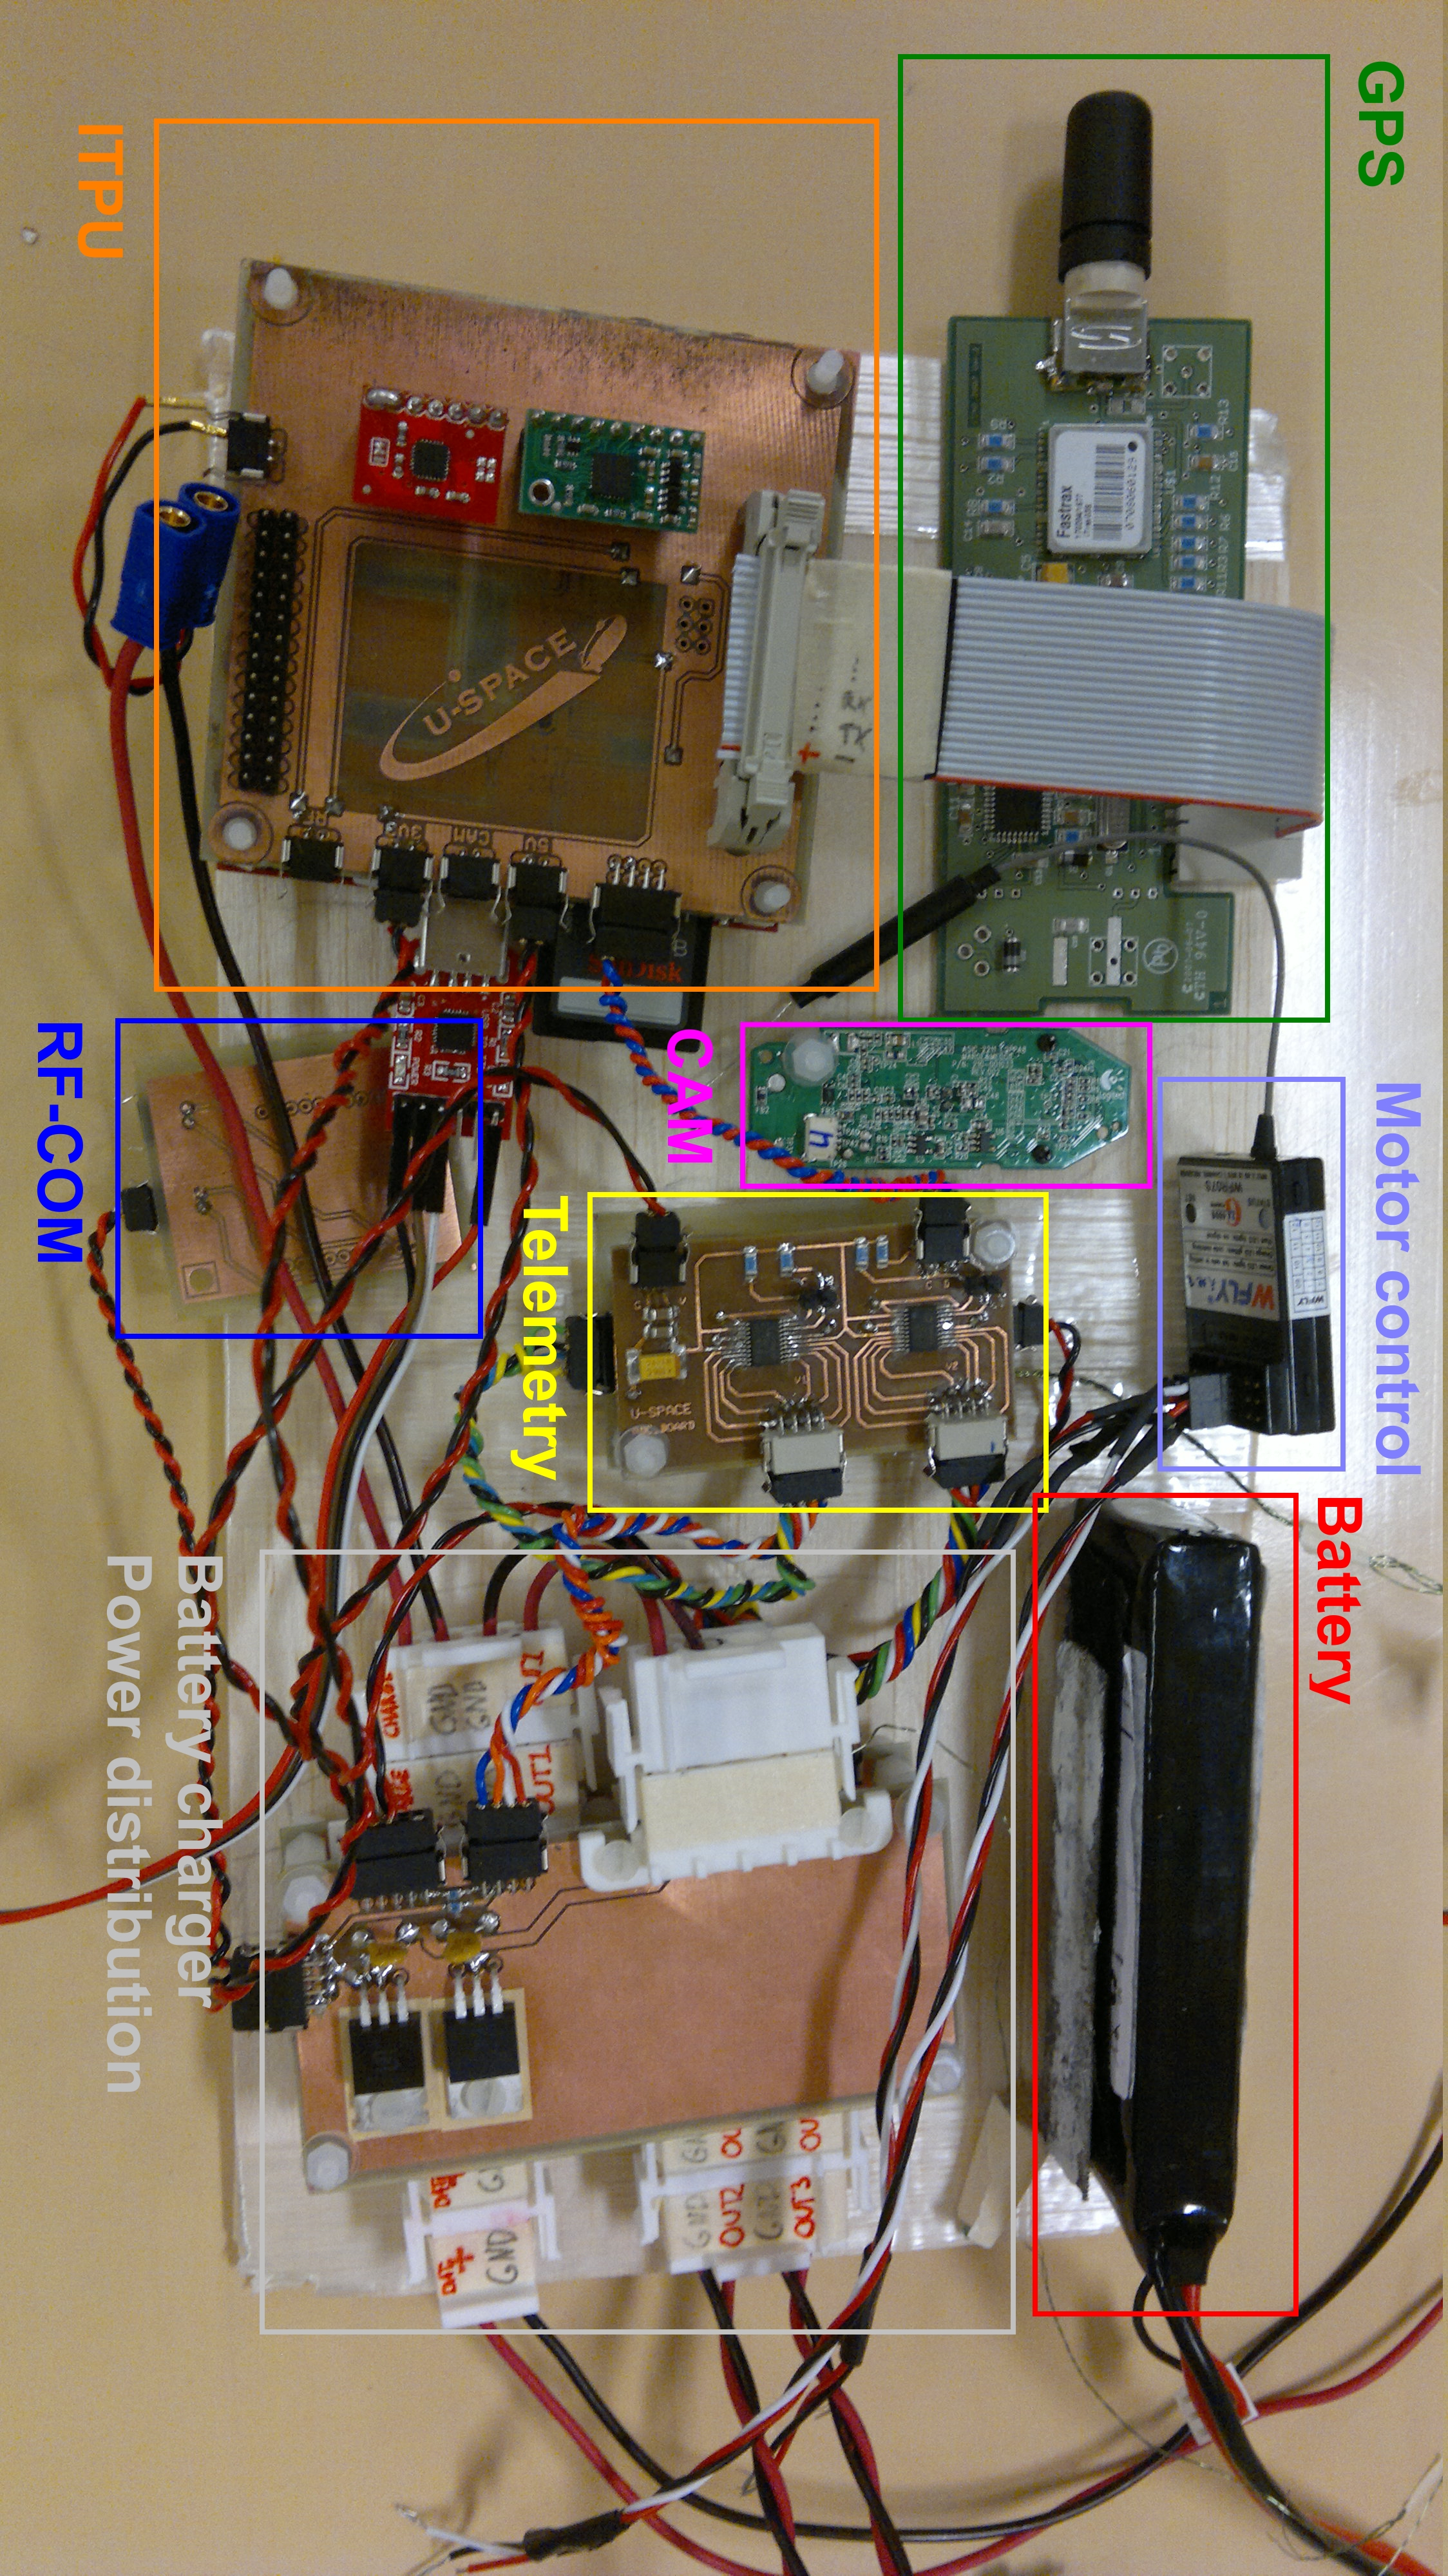
\includegraphics[width=0.55\textheight]{figures/full-system-setup}
\caption{Full system setup}
\label{fig:FlightTest1_1}
\end{figure}

An image of the full system setup including all electronical moduels can be seen in figure . This setup was then mounted into the payload box (see \textcolor{red}{REF!!!}) for testing. As mentioned in section \ref{sec:changes_itpu}, operating both the ADCs of the telemetry subsystem and the sensors of the attitude determination subsystem on the same I2C-bus caused problems which needed manual reset of the I2C-bus in order to get it working again. Peculiar was that both system worked when only one of the two ADCs where connected to the I2C bus together with the attitude sensors, but failed when both ADCs were connected. As the attempts to enable a second I2C-bus on a different expansion header of the BB were unsuccessful, it was decided to test only with one ADC and in turn loose 8 of the 16 telemetry values of the internal voltages. 

With this decision implemented the testing went successful. The wireless connection to the groundstation could be established (for more see \textcolor{red}{REF TO OMAIR}). After calibration of the magnetometer, the attitude determination system was able to determine the attitude stabily and produce the roll-, pitch- and yaw-angles for the telemetry system. When receiving the corresponding signal from the communication module the camera could be activated and shoot either single images or multiple images with a set period (fastest 1~s) and save them to the onboard sd-card.  
>>>>>>> 4fb6c5e283e39b3c694310944a6c6ff9cc25aad8

\begin{figure}
\centering
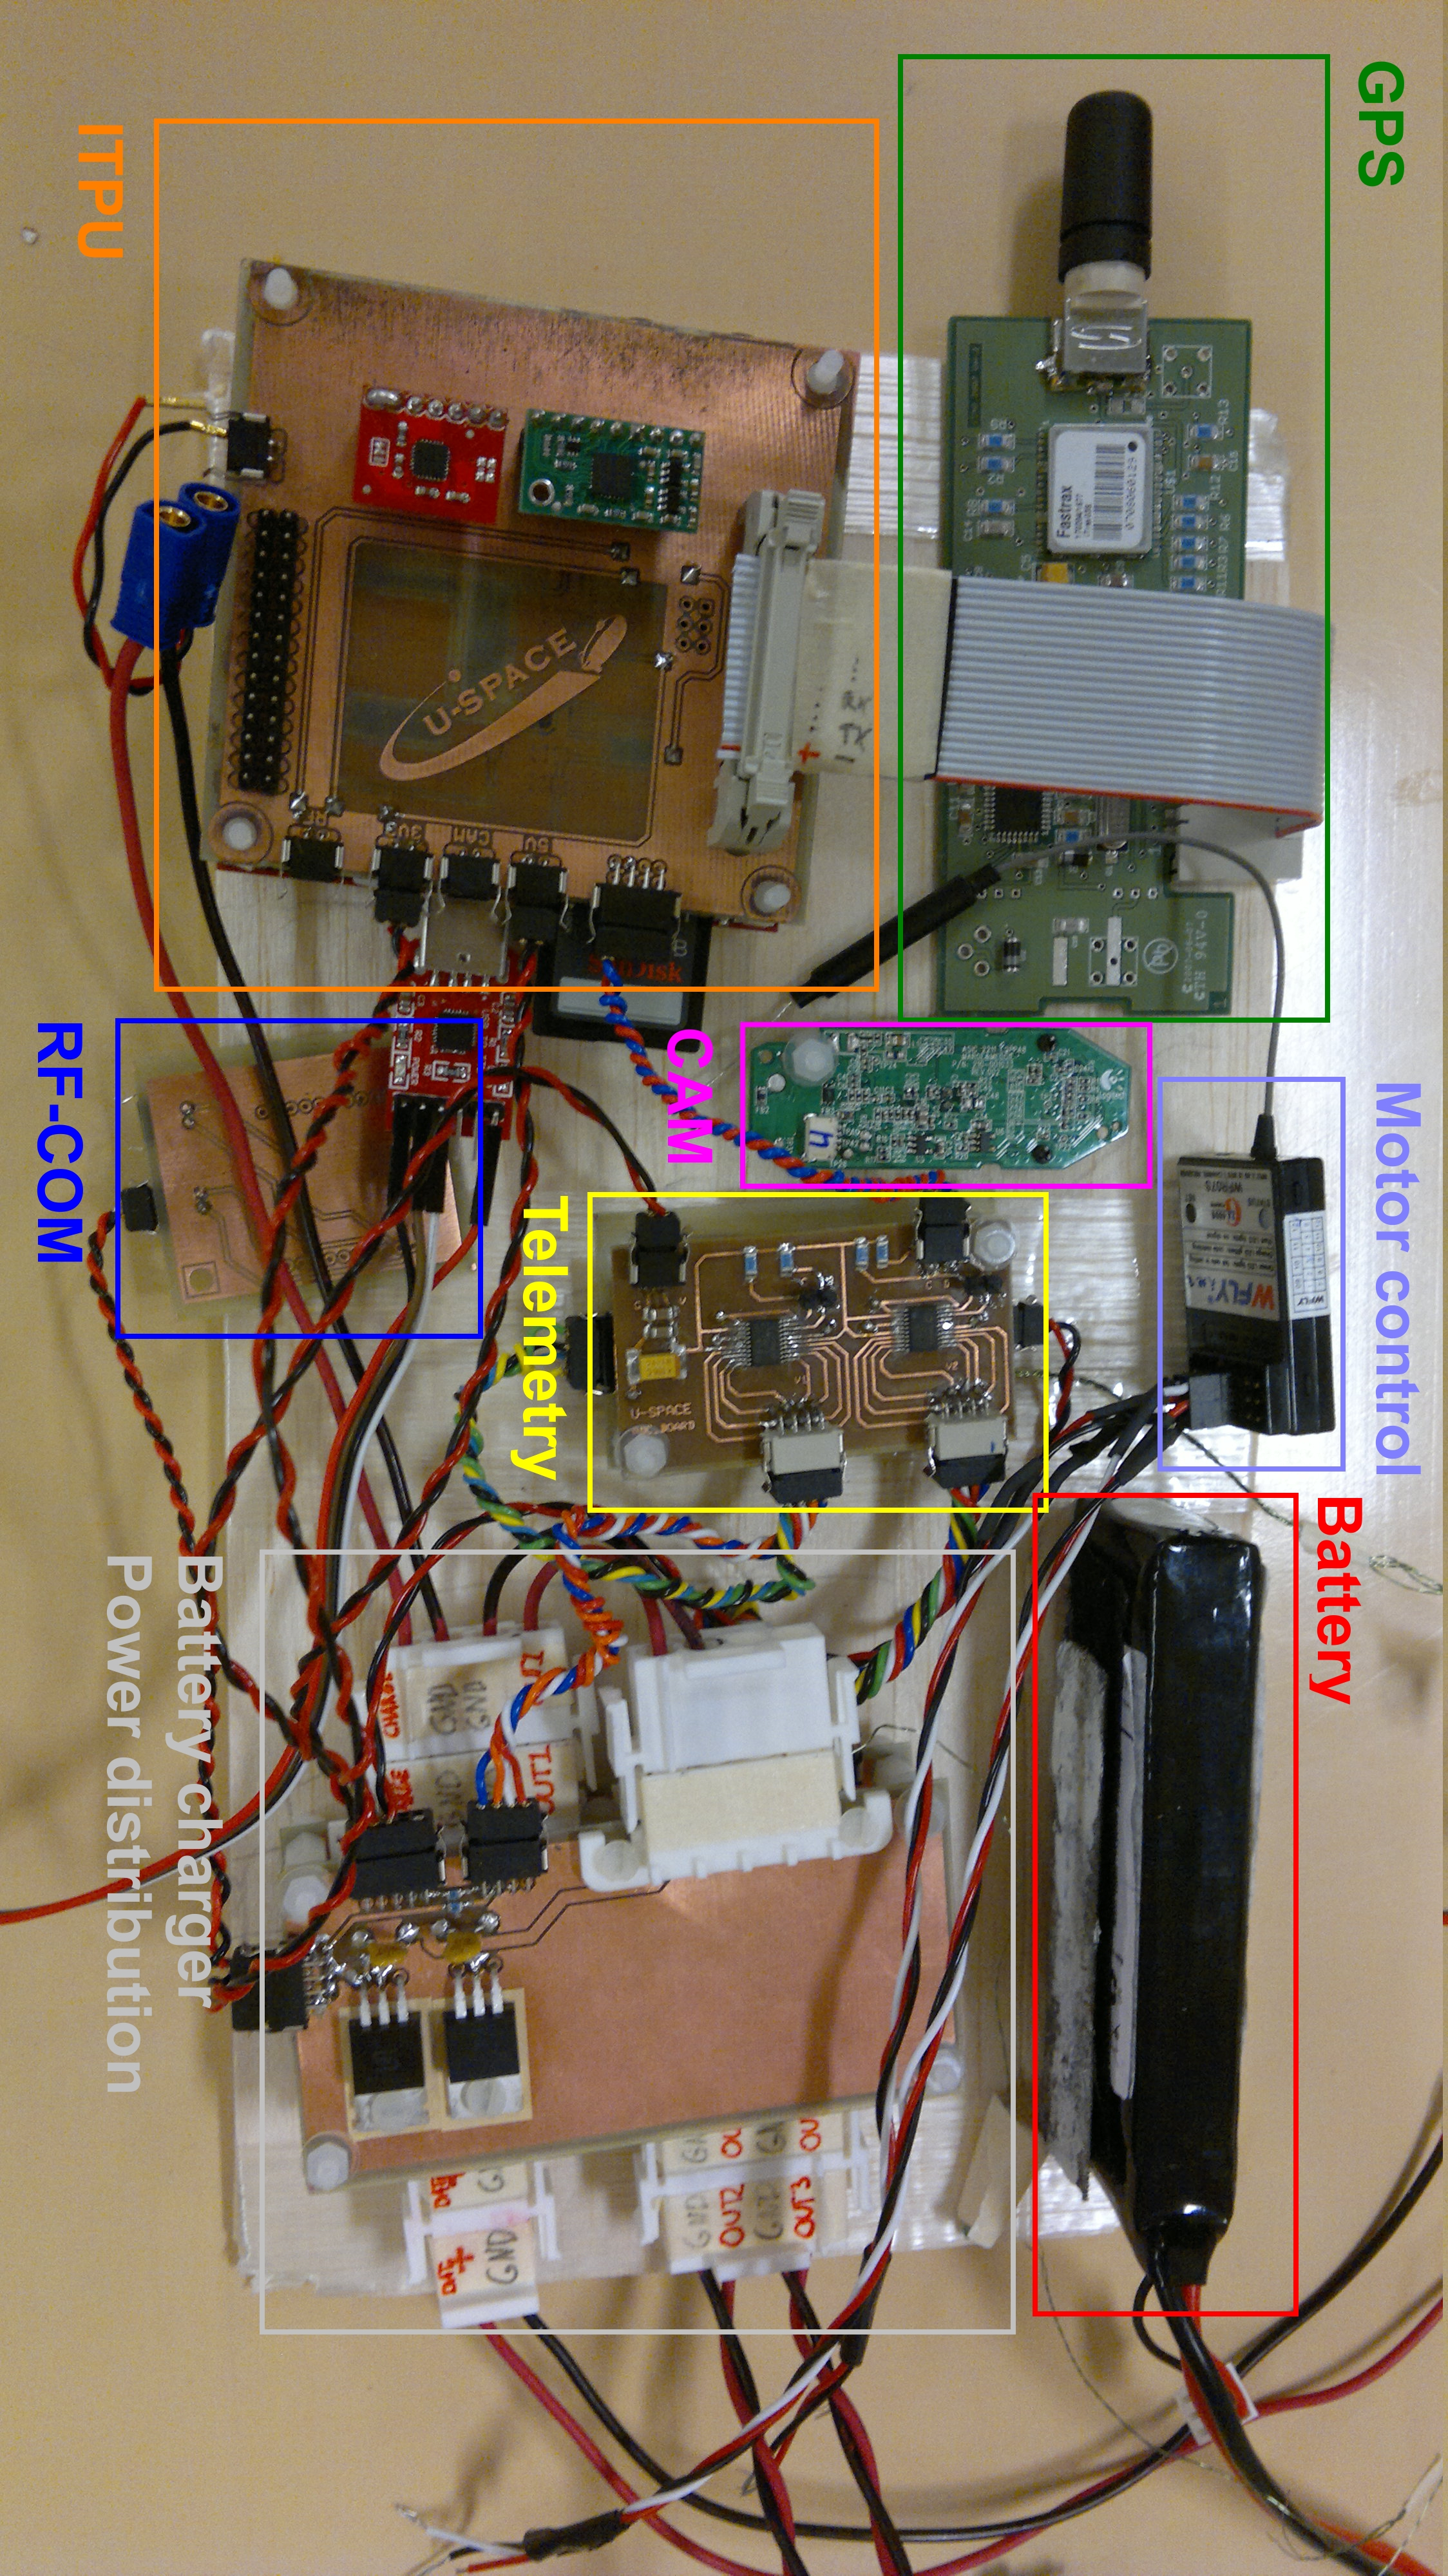
\includegraphics[width=0.55\textheight]{figures/full-system-setup}
\caption{Full system setup}
\label{fig:FlightTest1_1}
\end{figure}

An image of the full system setup including all electronical moduels can be seen in figure . This setup was then mounted into the payload box (see \textcolor{red}{REF!!!}) for testing. As mentioned in section \ref{sec:changes_itpu}, operating both the ADCs of the telemetry subsystem and the sensors of the attitude determination subsystem on the same I2C-bus caused problems which needed manual reset of the I2C-bus in order to get it working again. Peculiar was that both system worked when only one of the two ADCs where connected to the I2C bus together with the attitude sensors, but failed when both ADCs were connected. As the attempts to enable a second I2C-bus on a different expansion header of the BB were unsuccessful, it was decided to test only with one ADC and in turn loose 8 of the 16 telemetry values of the internal voltages. 

With this decision implemented the testing went successful. The wireless connection to the groundstation could be established (for more see \textcolor{red}{REF TO OMAIR}). After calibration of the magnetometer, the attitude determination system was able to determine the attitude stabily and produce the roll-, pitch- and yaw-angles for the telemetry system. When receiving the corresponding signal from the communication module the camera could be activated and shoot either single images or multiple images with a set period (fastest 1~s) and save them to the onboard sd-card.  

\section{Discussions and Future Recommendations}
%write for each subsystem
%
\subsection{EPS}
Due to the connector issues discussed in section \ref{sec:flight_results}, no telemetry was available during flight, thus detailed information of power consumption were not obtained. However, at full thrust, the system has in laboratory shown to draw around 2 x 7.5 A. At a voltage of approximately 7.0 V this corresponds to 105 W power delivered to the motors. In \cite{CDR} the \ac{EPS} was designed to deliver minimum 40 W of continuous solar power. With these flight results, to allow continuous flight, future designs should increase the solar array power output by at least a factor 2.5-3.
 
The \ac{BCR} should be re-designed for higher voltage and current outputs. Options for this were discussed in section \ref{sec:changes_BCR}. This also requires a battery pack with higher voltage. An advantage with higher voltage is that the power distribution efficiency is increased, since the diode voltage-drop losses and resistive losses ($I^2 \times R$) are relatively reduced when comparing to the total amount of handled power. 
%
\subsection{MCC}
From the previous discussed flight results, it was shown that the amount of generated thrust was just barely able to move the blimp. According to \cite{website:ModelMotors}, the motors have a relatively poor efficiency of around 67\%, especially when operating at heavy loads (high currents + low \ac{RMP}). The TIF-250 blimp from Esrange has a volume of $15 m^3$ and thus an approximate lift of around 15 kg. Including the motor efficiency, the power-to-lift ratio is 4.7 W/kg. Calculating this ratio for the Zeppelins that flew during the 1930's\cite{website:graf_zeppelin} gives 15.4 W/kg for the LZ-129 Hindenburg and 19.2 W/kg for the LZ-127 Graf. Thus the U-SPACE design has a power-to-lift ratio about 3-4 times less than old commercial designs. This agrees well with the lack of motor power to properly propel the blimp. The Zeppelins were designed for a cruise speed around 125 km/h (35 m/s) which is of course faster than the U-SPACE requirement. For future designs, it is recommended to include more powerful motors designed for low speed, low \ac{RPM} and high torque like \cite{website:ModelMotors_AXI5360}. Larger motors will also require a larger solar array to provide the power.

\newpage
\chapter{Project Evaluation}
\label{chap:evaluation}
% provide feedback about the project course: what was good/fun/etc.?, what did you learn?, what didn't work well?, what can be improved for future projects?, other comments...
%This is mainly for feedback to Thomas, Kjell and LTU.


\section{Pedro}


\section{Omair}


\section{Jan}


\section{Morten}
Establishment of Viking room to be permanent project course room. 
Quicker release of initial project budget to allow first order of components. 
Access to workshop and help from Lars worked very well.
Generally good support from IRF with borrowing tools and suggestions for mechanical design. If possible, more instructions and recommendations from IRF experts would have been a help (soldering course, how to check solderings under microscope).
More critical design feedback and suggestions from supervisors, where possible, would be appreciated.
More clear initial communication of project course requirement in terms of reports and presentations (how many, which and when).
\newpage
\chapter{Future Visions}
\label{chap:visions}
% future project visions for U-SPACE
%
It is the authors's believe that designing and building an airship is a great way for students to gain initial practical experiences on project work subjected to many of the same technical constraints also found in real space projects, including:
%
\begin{itemize}
\item Very limited power budget
\item Strong mass constraints due to limited lift mass
\item Thermal constraints considering daily and seasonal weather conditions, when flying outdoors
\item System autonomy, since no physical access to systems is possible once flying in the sky
\item Support requirements for scientific payloads
\item Mechanical structure optimized for low weight with strength and rigidity to withstand non-nominal situations (uncontrolled landings etc.)
\end{itemize}
%
Airships provide low cost and frequent flight opportunities thus allowing flight experience for all students involved in the project, even if only for a single semester.  Furthermore, if means are added to reuse helium gas after flight, one of the main expenses in these systems, flight costs can be reduced to almost zero.
Due to the recent popularity of private \ac{RC}-planes, many airship components can be found at low cost and high quality such as Li-ion batteries, motors, propellers and motor controllers.
\\\\
%
\noindent
The U-SPACE project has shown the way for many possible future upgrades which can be realized in student projects, including (but not limited to): 
%
\begin{itemize}
\item Realizing a completely solar powered flight in outdoor conditions.
\item Designing and building a custom envelope optimized for low weight and mechanical properties (rigidity, mounting options, ease of manufacturing etc.)
\item Altitude control system. This could be realized by having a compressor and an air-filled envelope. When inflating the air-filled envelope, it will compress the helium envelope thus reducing the lift of the airship (same concept as used on the old Zeppelins).
\item Attitude and flight path control system. Possibility to add coordinates and positions that the airship should automatically follow or maintain.
\item System up-scaling: Higher motor power, more lift capability to support larger and more sophisticated scientific payloads.
\item Scientific payloads: Atmospheric measurements (ice crystals, meteorological etc.), simple Synthetic Aperture Radar(as demonstrated by MIT lecturer in Optics and Radar course), space elevator demonstrator,...
\item Ground link with LTU ground station. Thus providing a professional high-bandwidth communication link and a test environment for students to gain experience as ground controllers who could then also support international cubesat missions around the globe.
\end{itemize}

\newpage
\printbibliography
\markboth{Bibliography}{Bibliography}
\addcontentsline{toc}{chapter}{\protect\numberline{}References}
\newgeometry{margin=1.5cm}
\pagestyle{plain}

%\begin{appendices}

\section{Some Appendix}\label{app:SomeAppendix}
some text...

\end{appendices}

\end{document}